\chapter{Felhasználói dokumentáció}
\label{ch:user}


\section{A szoftver célja}

Az alkalmazásnak három fő célja van:
\begin{enumerate}
    \item Biztosítani egy szerkesztőt, amivel bármilyen 2D-s sokszög elkészíthető.
    \item Lehetőséget adni arra, hogy az elkészített alazatra lefuttassuk az algoritmust.
    \item Személyreszabható és látványos módon vizualizáni a kiértékelt távolságfüggvényt
\end{enumerate}


\section{Hardveres és szoftveres követelmények}

\textbf{Hardver}
\begin{itemize}
    \item x86-64 architektúrájú CPU (Modern Intel vagy AMD processzorok többsége)
    \item DirectX 12 API kompatibilis GPU
    \item 8GB RAM
    \item billentyűzet, egér, monitor
\end{itemize}

\textbf{Szoftver}
\begin{itemize}
    \item Operációs rendszer: Windows 11
    \item DirectX 12 API kompatibilis GPU driver
\end{itemize}


\section{Telepítés és futtatás}

A program nem rendelkezik telepítővel, a mellékelt állomány kicsomagolása után a \textit{,,PolygonSDF.exe"} futtatásával azonnal használható. A mellékelt fájlok és mappák (pl. \textit{Falcor.dll}, \textit{Shaders/}, \textit{Data/}, ...) szükségesek az alkalmazás megfelelő működéséhez.


\section{Szerkesztői nézet}

Az alkalmazás indítása után a felhasználót a szerkesztői nézet fogadja, amelyben egy előre meghatározott alakzat jelenik meg. Egy alakzat több poligonból áll, minden poligont annak csúcspontjaival adjuk meg, ahol a megadási sorrend határozza meg azt, hogy hogy kötjük őket össze. A távolság előjelét az határozza meg, hogy az adott pont páros vagy páratlan számú sokszögön belül van-e, ami páros esetén pozitív és páratlan esetén negatív távolságot eredményez.

A szerkesztőben lehetőségünk van poligonok felvételére, mozgatására és törlésére, valamint csúcspontjaik módosítására. Ezen műveleteket kétféle módon is elvégezhetjük, a vizuális szerkesztővel, a billentyűzet és egérmozdulatok segítségével, vagy a GUI-n elhelyezett beviteli mezőkkel és gombokkal. Amikor elkészültünk a szerkesztéssel, az algoritmust is ezen felületen keresztül futtathatjuk le.

\begin{figure}[H]
    \centering
    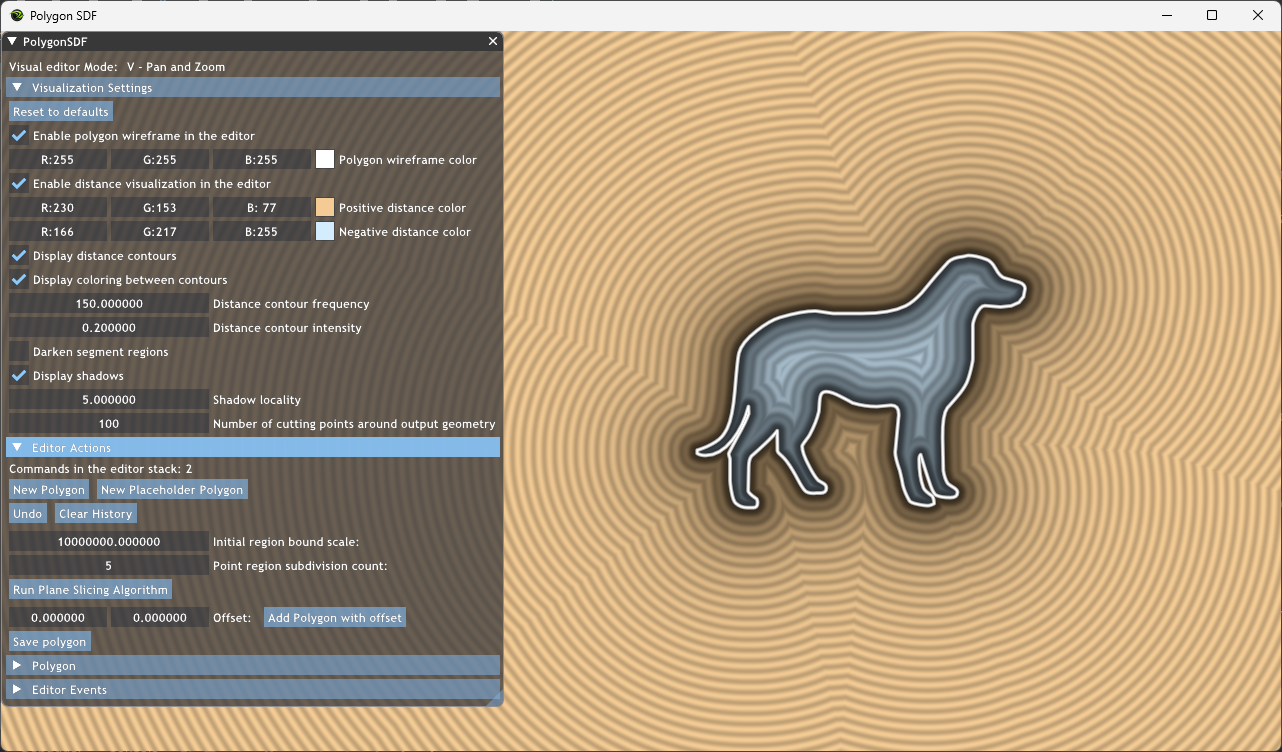
\includegraphics[width=1\linewidth]{images/editor.png}
    \caption{Szerkesztői nézet}
    \label{fig:editor-1}
\end{figure}

\section{GUI szerkesztő}

Lehetővé teszi, hogy pontos értékekkel dolgozzunk a szerkesztés közben, mivel beviteli mezőkkel és gombokkal adunk ki parancsokat kattintások helyett a vásznon.
Ezért GUI szerkesztő központi szerepet tölt be az alkalmazás használatában, bizonyos műveleteket csak itt lehet végrehajtani, mint például a vizualizációs beállítások módosítása, algoritmus lefuttatása, mentés és betöltés. Itt kerül megjelenítésre az is, hogy a vizuális szerkesztő milyen módban van.

A GUI szerkesztő csoportokra van felosztva, az elvégzett feladatkör szerint.


\subsection{Vizualizációs beállítások}

A \ref{fig:visualization_settings-1}-es ábrán látható menüben állíthatjuk be az objektumunk megjelenítését. Bizonyos tulajdonságok, mint például a színezés, árnyékolás, vagy kontúrozás, mindkét nézetben érvényesülnek.

\begin{figure}[H]
    \centering
    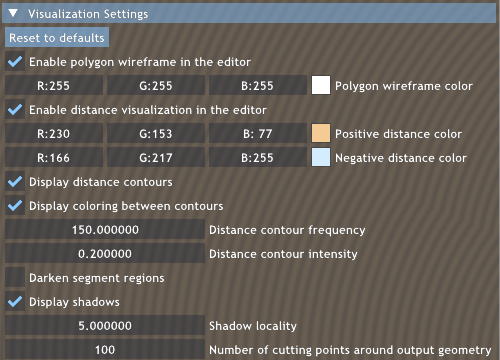
\includegraphics[width=0.8\linewidth]{images/visualization_settings.png}
    \caption{Vizualizációs beállítások GUI}
    \label{fig:visualization_settings-1}
\end{figure}

\textbf{Elérhető beállítások}

\begin{description}
    \item[Enable polygon wireframe in the editor] \textit{Körvonal engedélyezése} -- Ki- és bekapcsolhatjuk az alakzat körvonalának megjelenítését.
    \item[Polygon wireframe color] \textit{Körvonal szín} -- Kiválaszthatjuk, hogy milyen RGB értékkel kerüljön kirajzolásra a körvonal.
    \item[Enable distance visualization in the editor] \textit{Távolság megjelenítése} -- Szabályozhatjuk, hogy az alkalmazás rajzolja-e a távolságot. Ez egy viszonylag drága beaállítás, mert a minden kiszínezett pixelre a képernyőn ki kell értékelni a távolságot.
    \item[Positive distance color] \textit{Távolság pozitív tartományának színe} -- Megadhatjuk, hogy a pozitív tartomány színezésekor milyen alapszínt használjon a program
    \item[Negative distance color] \textit{Távolság negatív tartományának színe} -- Megadhatjuk, hogy a negatív tartomány színezésekor milyen alapszínt használjon a program
    \item[Display distance contours] \textit{Távolsági kontúrok megjelenítése} -- A beállított értékkel megszabhatjuk, hogy mekkora területre terjedjen ki az árnyék. Nagyobb érték esetén az árnyékolt rész kisebb, gyorsabban veszít az intenzitásából, ahogy a távolság növekedik.
    \item[Display coloring between contours] \textit{Kontúrok közötti tartomány kitöltése} -- Ezzel a beállítással látványosabbá tehetjük azt, hogy egy adott pontban az alakzat egy éléhez, vagy egy csúcsához van-e közelebb. Az élekhez közelebbi pontokhoz tartozó pixelek sötétebb színt kapnak.
    \item[Distance contour frequency] \textit{Távolsági kontúrvonalak frekvenciája} -- Kontúrok megjelenítésének szabályozása.
    \item[Distance contour intensity] \textit{Távolsági kontúrvonalak intenzitása} -- Beállítás a kontúrok közötti tartomány színezésére. Amennyiben le van tiltva a kontúrok közötti terület nem kerül színezésre.
    \item[Display shadows] \textit{Árnyék megjelenítése} -- A távolság megjelenítéséhez használt kontúrvonalak gyakorisága. A magasabb megadott érték sűrűbben elhelyezkedő kontúrvonalakat eredményez.
    \item[Shadow locality] \textit{Árnyék lokalitása} -- Megadja, hogy színezéskor mennyivel súlyozzuk a kontúr színét a háttérhez képest. Nulla értékű intenzitással nincsenek kontúrvonalak, egy értéknél pedig nincs színezés közöttük.
    \item[Darken segment regions] \textit{Élekhez tartozó régiók elsötétítése} -- Ki- és bekapcsolhatjuk az árnyékok rajzolását az alakzat körvonala mentén. A háromdimenziós nézetben fontos szerepe van az árnyéknak, mert információt ad a geometria mélységéről.        \item[Number of cutting points around output geometry] \textit{Az algoritmus kimenetének körbevágásához használt pontok száma} -- Az algoritmus egy \textit{,,végtelenül nagy"} síkkal dolgozik. Megjelenítés előtt ezt a síkot az alkalmazás az alakzat középpontja körül egy az alakzat méretétől függő sugarú körív mentén körbevágja. A beviteli mezővel a vágáshoz használt pontok számát szabályozhatjuk.
\end{description}

\begin{figure}[H]
    \centering
    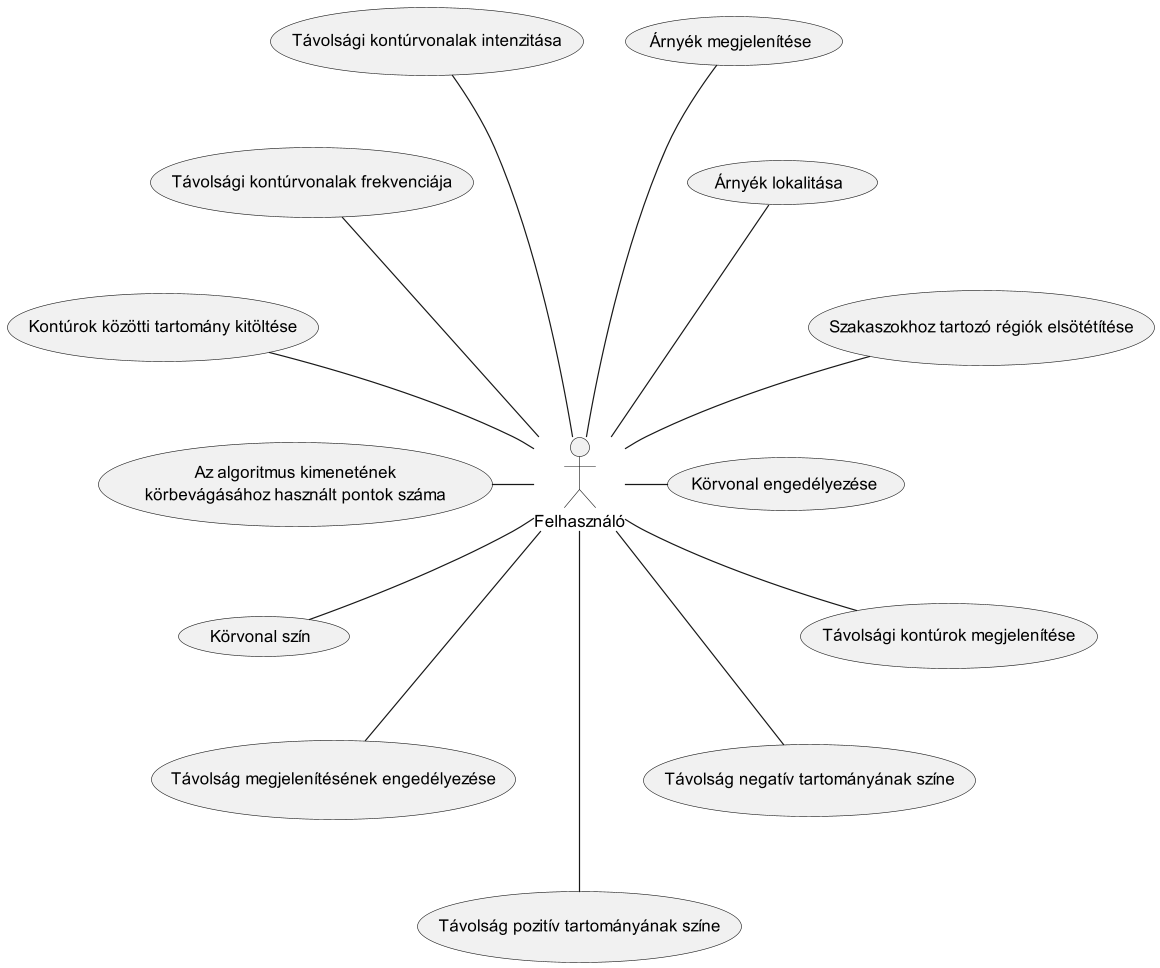
\includegraphics[width=1\linewidth]{images/usecase_visualization_settings.png}
    \caption{Vizualizációs beállítások felhasználói esetek}
    \label{fig:usecase_visualization_settings-1}
\end{figure}

\begin{figure}[H]
    \centering
    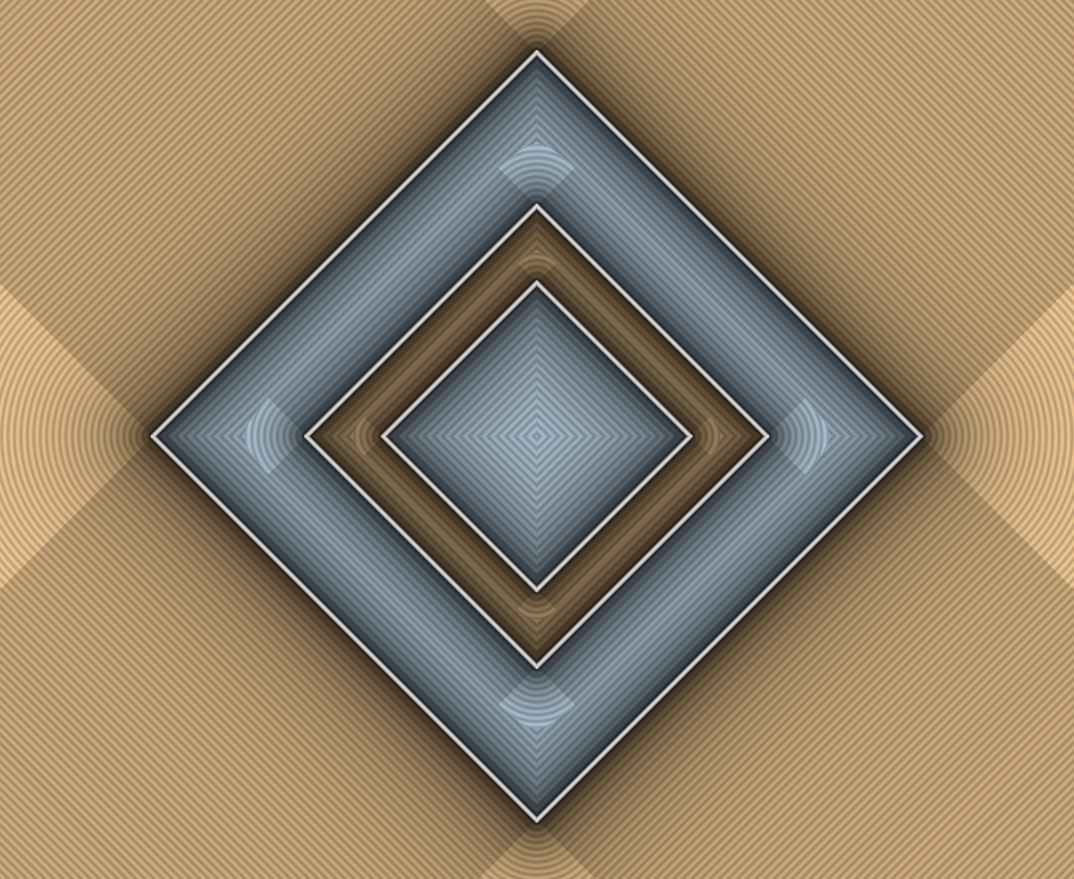
\includegraphics[width=0.85\linewidth]{images/darken_segment_regions.png}
    \caption{Élekhez tartozó régiók elsötétítése}
    \label{fig:darken_segment_regions-1}
\end{figure}

\begin{figure}[H]
    \centering
    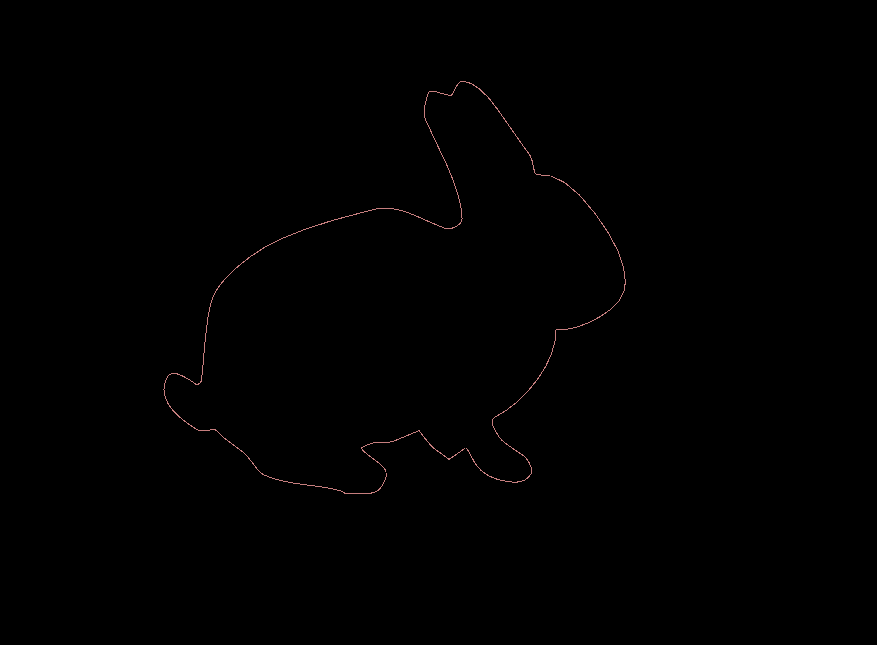
\includegraphics[width=0.85\linewidth]{images/outline_only.png}
    \caption{Alakzat ,,wireframe" nézete}
    \label{fig:outline_only-1}
\end{figure}

\begin{figure}[H]
    \centering
    
\includegraphics[width=0.78\linewidth]{images/hidden_contours.png}
    \caption{Megjelenítés kontúrok nélkül}
    \label{fig:hidden_contours-1}
\end{figure}

\begin{figure}[H]
    \centering
    
\includegraphics[width=0.78\linewidth]{images/low_shadow_locality.png}
    \caption{Megjelenítés alacsony árnyék lokalitással}
    \label{fig:low_shadow_locality-1}
\end{figure}

\begin{figure}[H]
    \centering
    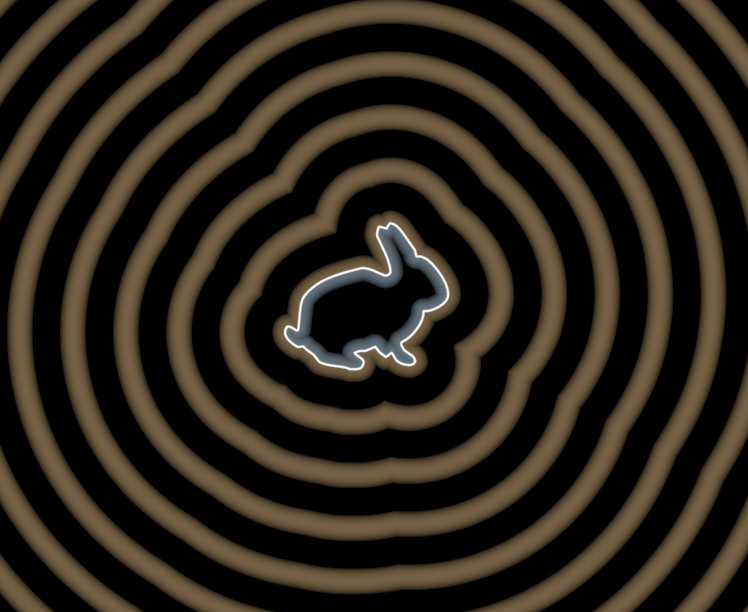
\includegraphics[width=0.85\linewidth]{images/low_contour_frequency.png}
    \caption{Megjelenítés alacsony kontúr frekvenciával}
    \label{fig:low_contour_frequency-1}
\end{figure}

\begin{figure}[H]
    \centering
    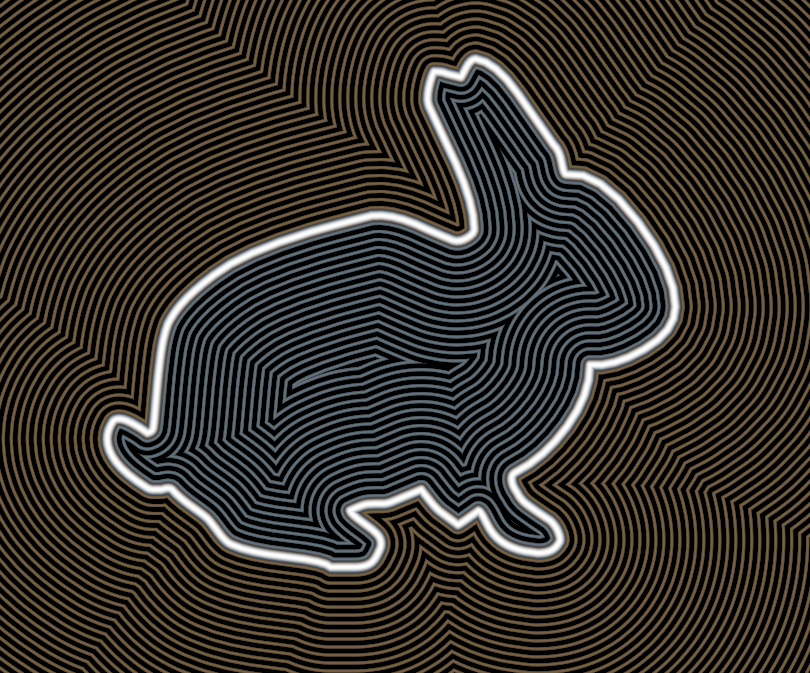
\includegraphics[width=0.85\linewidth]{images/high_contour_frequency.png}
    \caption{Megjelenítés magas kontúr frekvenciával}
    \label{fig:high_contour_frequency-1}
\end{figure}

\subsection{Szerkesztői műveletek}

A \ref{fig:editor_actions-1}-es ábrán látható menüben általános szerkesztői műveletek találhatóak, mint például adatok betöltése, mentése, algoritmus futtatása. A szerkesztő az állapotokat veremszerűen tárolja, új művelet hozzáadásakor beszúrunk egy új bejegyzést, visszalépéskor pedig kiveszünk egyet. Ez a funkció szabadságot ad a felhasználónak kísérletezésre, mivel bármikor visszaléphet az arra szánt gomb megnyomásával, viszont a műveletek számával növekszik a memóriaigénye is a programnak, ezen a felületen keresztül törölhetjük is a szerkesztői előzményeket.

\begin{figure}[H]
    \centering
    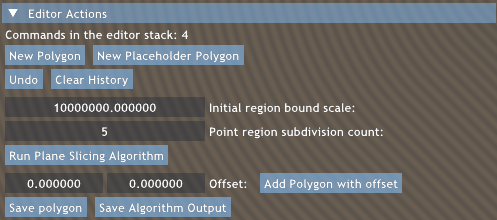
\includegraphics[width=0.85\linewidth]{images/editor_actions.png}
    \caption{Szerkesztői műveletek GUI}
    \label{fig:editor_actions-1}
\end{figure}

\textbf{Elérhető funckionalitás}

\begin{description}
    \item[New shape] \textit{Új alakzat hozzáadása} -- A fáljrendszerből tölt be egy sokszöget a meglévőt lecserélve, amennyiben a megadott JSON file a megfelelő formátumban van, ellenkező esetben egy felugró ablakkal értesül a felhasználó, hogy a művelet sikertelen.
    \item[Set to starter shape] \textit{Alakzat beállítása a kezdőalakzatra} -- A jelenlegi alakzatot lecseréli a kezdőalakzatra.
    \item[Undo] \textit{Visszalépés} -- Az utolsó lépés visszavonása, amennyiben lehetséges.
    \item[Clear history] \textit{Előzmények törlése} -- A szerkesztői előzmények törlése, a köztes állapotokra fenntartott memória felszabadításához.
    \item[Run Plane Slicing Algorithm] \textit{A vágásokat végző algoritmus futtatása} -- Ha az alakzat megfelel az algoritmus előfeltételének, tehát nincsenek egymást metsző vagy egymásba eső élek, akkor az alkalmazás végrehajtja. Ellenkező esetben egy felugró ablak jelzi, hogy a művelet sikertelen.
    \item[Add Shape With Offset] \textit{Alazkat hozzáfűzése eltolással} -- A fáljrendszerből tölt be egy sokszöget a meglévőhöz hozzáfűzve azt, a megadott X és Y koordinátákkal eltolva. Amennyiben a megadott JSON file a megfelelő formátumban van, ellenkező esetben egy felugró ablakkal értesül a felhasználó, hogy a művelet sikertelen.
    \item[Save shape] \textit{Alakzat mentése} -- A szerkesztett alakzat jelenlegi állapotát a fáljrendszerbe menti JSON formátumban.
    \item[Save Algorithm Output] \textit{Algoritmuskimenet mentése} -- Az alakzathoz tartozó algoritmuskimenetet lementi a fáljrendszerbe menti JSON formátumban, ha az algoritmus végre lett hajtva, ellenkező esetben nem kerül megjelenítésre a gomb.
\end{description}

\begin{figure}[H]
    \centering
    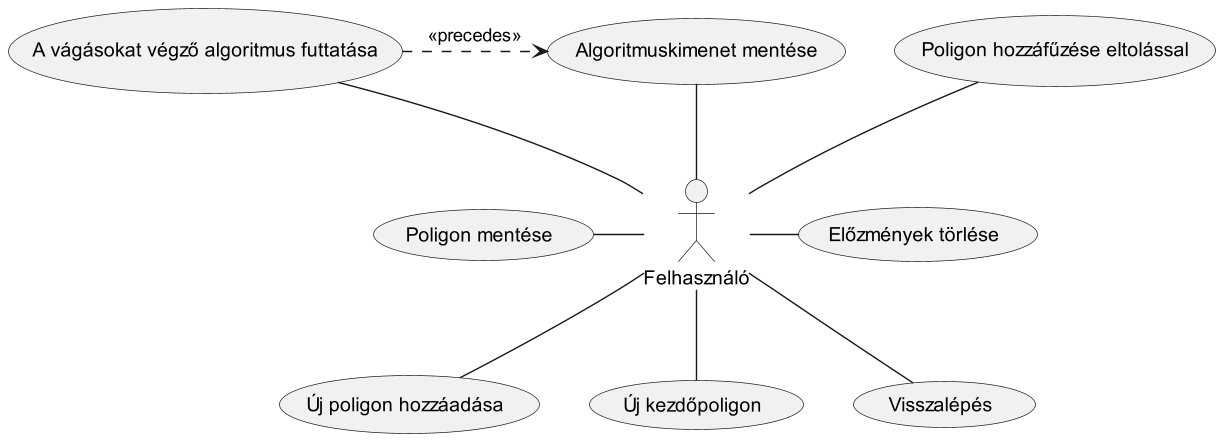
\includegraphics[width=1\linewidth]{images/usecase_editor_actions.png}
    \caption{Szerkesztői műveletek felhasználói esetek}
    \label{fig:usecase_editor_actions-1}
\end{figure}

\subsection{Alakzat műveletek}

A \ref{fig:shape_actions-1}-es ábrán látható menüben az alakzat tartalmának módosítására létrehozott műveletek találhatóak.

\begin{figure}[H]
    \centering
    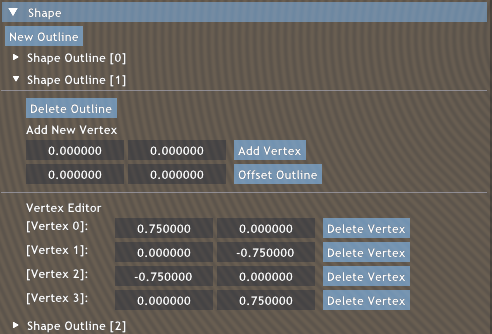
\includegraphics[width=0.85\linewidth]{images/shape_actions.png}
    \caption{Alakzat műveletek GUI}
    \label{fig:shape_actions-1}
\end{figure}

\textbf{Elérhető funckionalitás}

\begin{description}
    \item[New Outline] \textit{Új poligon hozzáadása} -- Egy új poligon kerül hozzáadásra. Az új poligon felhasználható lyukak vagy további elkülönülő alakzat elkészítésére.
    \item[Shape Outline > Delete Outline] \textit{Poligon > Poligon törlése} -- Törli az adott poligont, azzal a feltétellel, hogy egy alakzatban legalább egy poligonnak szerepelnie kell.
    \item[Shape Outline > Add Vertex] \textit{Poligon > Csúcs hozzáadása} -- A megadott pozícióval hozzáad egy csúcspontot a poligon végére.
    \item[Shape Outline > Offset Outline] \textit{Poligon > Poligon eltolása} -- A megadott pozícióval eltolja minden csúcsát a poligonnak.
    \item[Shape Outline > Vertex > Delete Vertex] \textit{Poligon > Csúcs > Törlés} -- Eltávolítja az adott csúcsot.
\end{description}

\begin{figure}[H]
    \centering
    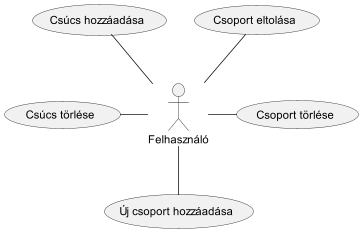
\includegraphics[width=.6\linewidth]{images/usecase_polygon_actions.png}
    \caption{Alakzat műveletek felhasználói esetek}
    \label{fig:usecase_polygon_actions-1}
\end{figure}

\subsection{Eseménynapló}

A szerkesztés során számos esemény kerül kiváltásra különböző források hatására. A \ref{fig:editor_events-1}-es ábrán látható eseménynaplóban megvizsgálhatunk minden bejövő eseményt valós időben. Az ismétlődő szignatúrák számozással csoportosításra kerülnek, mivel bizonyos esetekben másodpercenként akár több tíz is kiváltódhat, például amikor a felhasználó az egérrel mozgat egy csúcspontot, vagy egy poligont.

\begin{figure}[H]
    \centering
    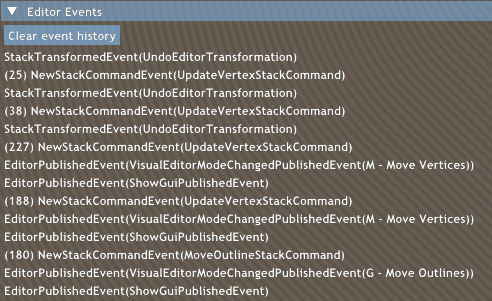
\includegraphics[width=1\linewidth]{images/editor_events.png}
    \caption{Eseménynapló GUI}
    \label{fig:editor_events-1}
\end{figure}


\textbf{Elérhető funckionalitás}

\begin{description}
    \item[Clear History] \textit{Napló törlése} Az összes bejegyzés törlése a naplóból.
\end{description}

\subsection{Parancslista}

A \ref{fig:user_guide-1}-ös ábrán látható felületen megtekinthetjük az összes elérhető billentyűparancsot a szerkesztőprogramhoz.

\begin{figure}[H]
    \centering
    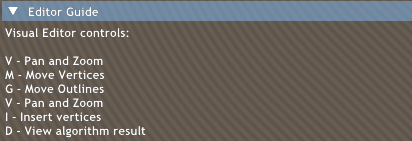
\includegraphics[width=1\linewidth]{images/user_guide.png}
    \caption{Parancslista GUI}
    \label{fig:user_guide-1}
\end{figure}


\section{Vizuális szerkesztő}\label{sec:visual_editor}

A vizuális szerkesztő lehetőséget ad arra, hogy szabadkézzel szerkesszük a sokszögünket. Billentyűzet segítségével válthatunk módok (eszközök) között, majd az egérrel interakcióba léphetünk az alakzattal vagy a vászonnal. A vizuális szerkesztőn keresztül válthatunk a háromdimenziós nézetre is.

\textbf{Elérhető funckionalitás}

\begin{description}
    \item[Csúcspontok mozgatása (M billentyű)] Csúcspontok ,,Drag and drop" mozgatása. Egérgomb lenyomásakor a program kiválasztja a legközelebbi csúcspontot egy megadott távolságkorláton belül és mozgatás hatására frissíti a pozíciójat.
    \item[Poligon mozgatása (G billentyű)]  Poligonok ,,Drag and drop" mozgatása. Egérgomb lenyomásakor a program kiválasztja a legközelebbi csúcsponthoz tartozó poligont egy megadott távolságkorláton belül és mozgatás hatására frissíti a poligonban lévő csúcspontok pozícióját.
    \item[Vászon mozgatása (V billentyű)] Az egérgomb nyomvatartásával és mozgatással mozgatni lehet a vászonon a teljes alakzatot. A görgő segítségével pedig nagyítani és zsugorítani a méretén. Ez a művelet nem módosít az alakzat állapotán.
    \item[Csúcspont beszúrása (I billentyű)] A bal egérgomb lenyomásával elhelyez egy csúcspontot a kattintás pozíciójához legközelebbi kettő, azonos poligonhoz tartozó csúcspont közé. A jobb egérgomb lenyomásával a legközelebbi csúcspont törlésre kerül, amennyiben egy megadott távolságon belül van.
    \item[Váltás a háromdimenziós algoritmus kimenet nézetre (D billentyű)] Ha az algoritmus végrehajtásra került az alakzat jelenlegi állapotán, akkor átvált a háromdimenziós nézetre, egyébként egy felugró ablakban jelzi, hogy nincs mit megjeleníteni.
\end{description}

\begin{figure}[H]
    \centering
    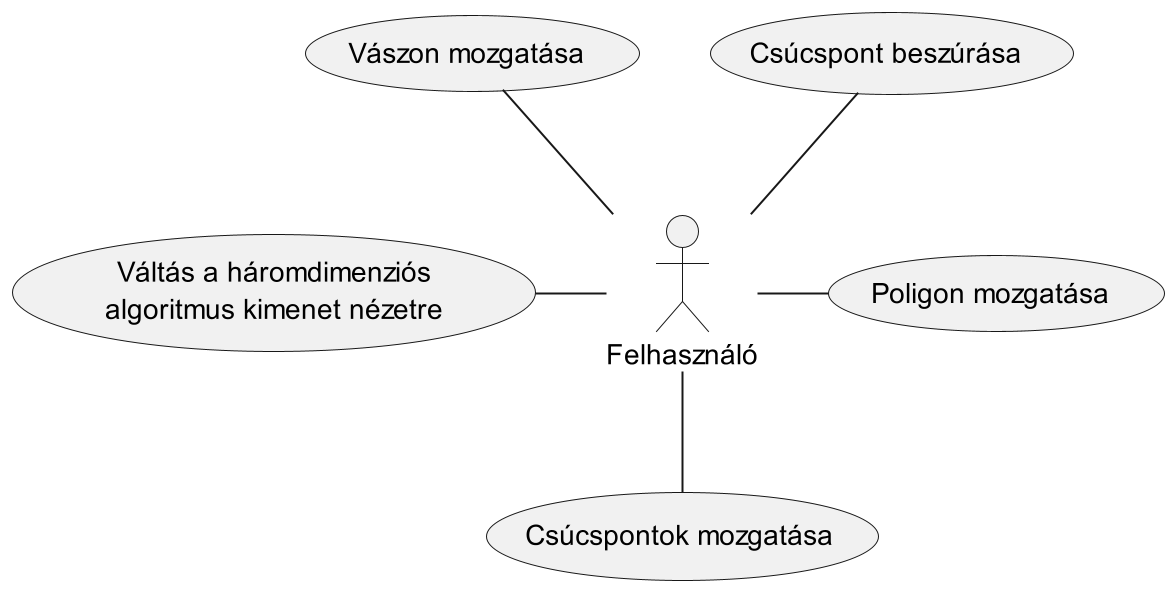
\includegraphics[width=.7\linewidth]{images/usecase_visual_editor.png}
    \caption{Vizuális szerkesztő felhasználói esetek}
    \label{fig:usecase_visual_editor-1}
\end{figure}

\section{Alakzat háromdimenziós nézete}

Az algoritmus kimenetével egy háromdimenziós objektumként számol az alkalmazás megjelenítéskor, ahol a mélységi komponens az előjeles távolság abszolútértéke. Ezt a tulajdonságot kihasználva ebben a nézetben a térben mozgatva tekinthetjük meg alakzatunkat.

Ebben az állapotban nem szerkeszthető az alakzat, ezért a teljes GUI el van rejtve. A szerkesztői felületre bármelyik \ref{sec:visual_editor}-ban említett eszközhöz rendelt billentyű lenyomásával átválthatunk.

\begin{figure}[H]
    \centering
    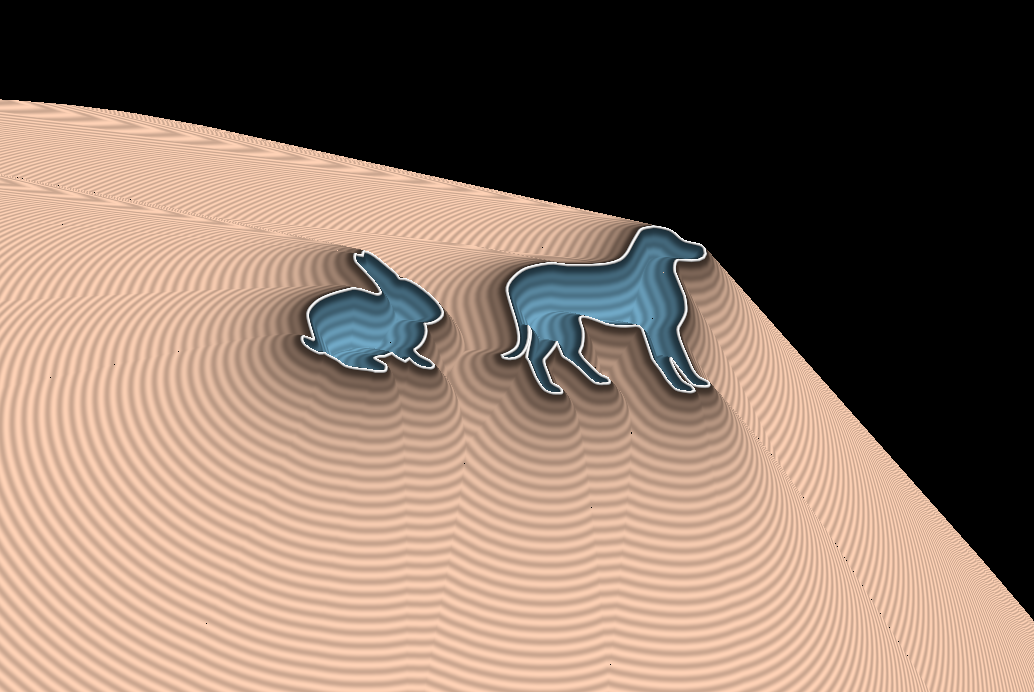
\includegraphics[width=1\linewidth]{images/3d_view.png}
    \caption{Alakzat háromdimenziós nézete}
    \label{fig:3d_view-1}
\end{figure}

A görgő segítségével változtathatjuk a távolságot a kamera és az objektum közepe között. Az egérgomb lenyomvatartása és mozgatással pedig forgathatjuk a geometriát, a mozgatás horizontális komponensével az Y tengey körül, a vertikális komponenssel pedig az X tengely körül.
